%! TeX program = xelatex
\documentclass[12pt, a4paper]{article}
\usepackage{geometry, tikz, float, pgfplots, xcolor, titlesec, amsmath, url, hanging, siunitx, graphicx, sectsty}
\usepackage[utf8]{inputenc}
\usepackage[skip=3pt]{parskip}
\usepackage[none]{hyphenat}
\usepackage[no-math]{fontspec}   % only changes normal font
% Tells LaTeX the images are kept in the "images" folder under the main directory
\graphicspath{ {./assets/} }
\pgfplotsset{compat=1.18, width=10cm}
% Spacing of sections: 0pt on the left, 18pt above, and 12pt below
\titlespacing\section{0pt}{18pt}{12pt}
% font size 12 for the sections
\sectionfont{\fontsize{12}{15}\selectfont}

% Setting font
\setromanfont{Arial}

% Setting strict margins
\sloppy

\begin{document}

\begin{center}

% Extra space at the top of the document
\noindent \\[10pt]
\color{black}

\thispagestyle{empty} % No page number for this page

\Large{\textbf{Properties of Gamma Radiation}} \\[30pt]
\normalsize \textit{Jack Greenberg, Jacob Fairham}\\[5pt]
\textit{11017146,  11074241}\\[20pt]
Department of Physics and Astronomy \\[5pt]
The University of Manchester \\[20pt]
First Year Laboratory Report 2 \\[20pt]
January 2023 \\[25pt]

\end{center}

\textbf{Abstract}\\[12pt]
This expirement aimed to analyze the spectra created using gamma ray spectroscopy using thallium-activated sodium iodide scintillation detectors with radioactive isotopes such as $^{22}$Na, $^{60}$Co, and $^{137}$Cs. The peaks of the $^{22}$Na spectrum were then used to calculate the strength of the sodium source and the relative efficiencies of the detector at the different photopeak energies. Finally, different materials were used between the isotopes and the detector to measure the relation between gamma ray detections and the thickness of the barrier between the source and the detector at different energy levels. We found our isotope of $^{22}$Na had a source strength of $11.77\pm1.81$kBq, as compared to its theoretical $15.09$kBq obtained using the initial source strength as well as the half life of the isotope and the amount of time that has passed from the initial source measurement.

\noindent 

\pagebreak

\section{Introduction}
	<insert introduction here>

\section{Experimental Setup}
	<insert more stuff here>

\section{Interpreting the Spectra}
	this is how you would include a graph!
	\begin{figure}[H] \centering
		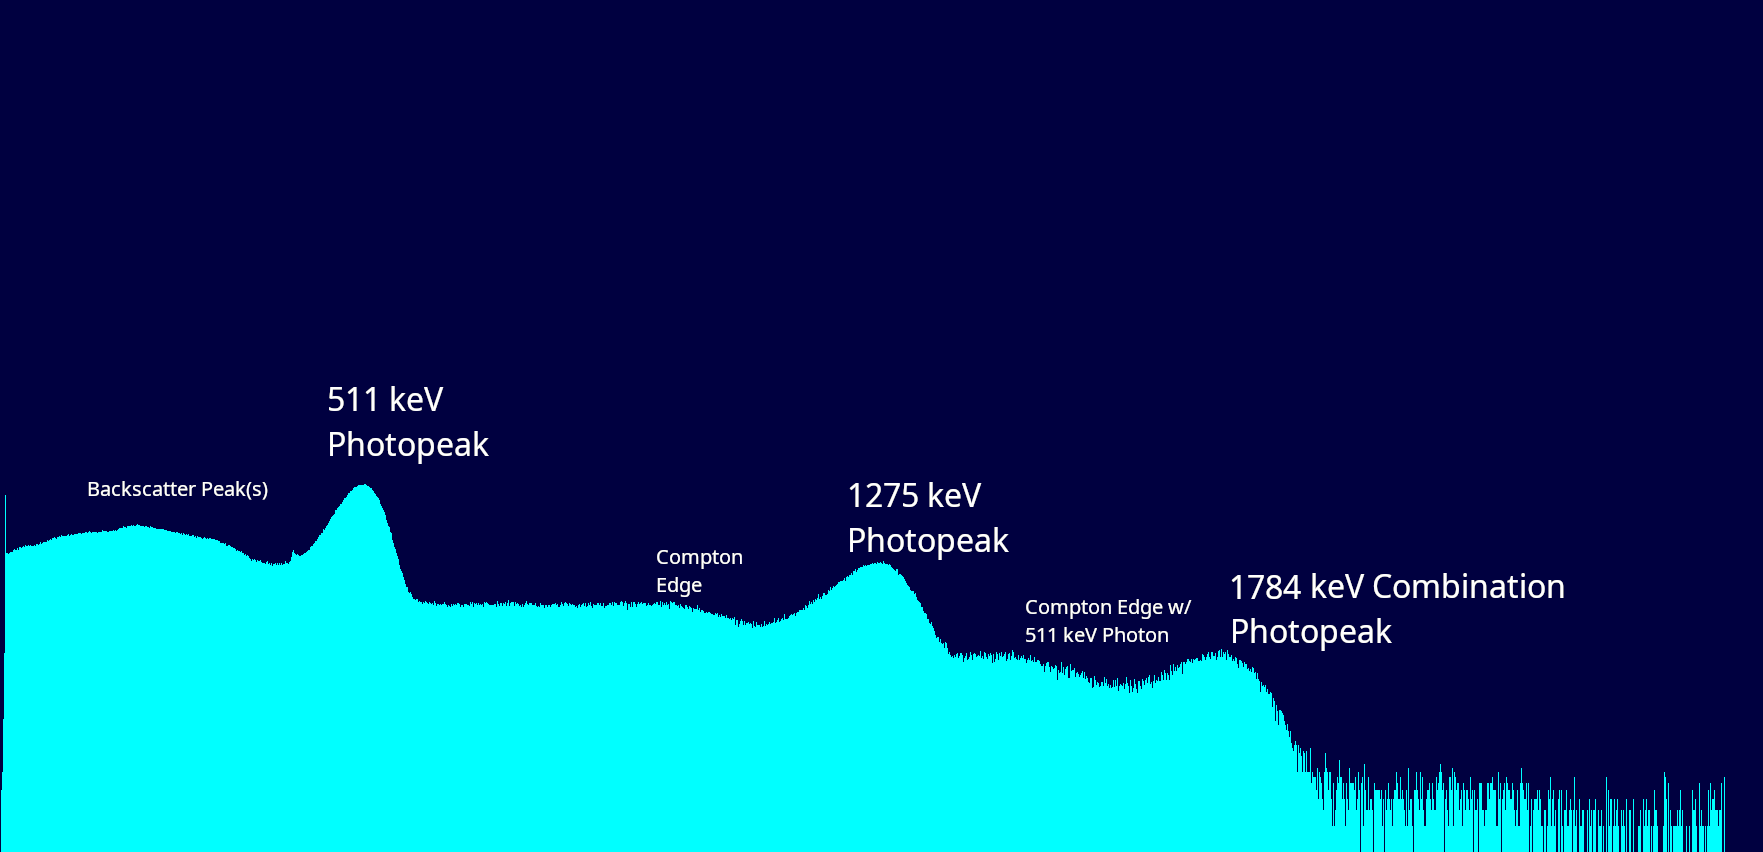
\includegraphics[scale=0.3]{assets/na22_log_annotated.png}
		\caption{Spectrum of Sodium 22 - Log scale counts by energy}
	\end{figure}
	\begin{figure}[H] \centering
		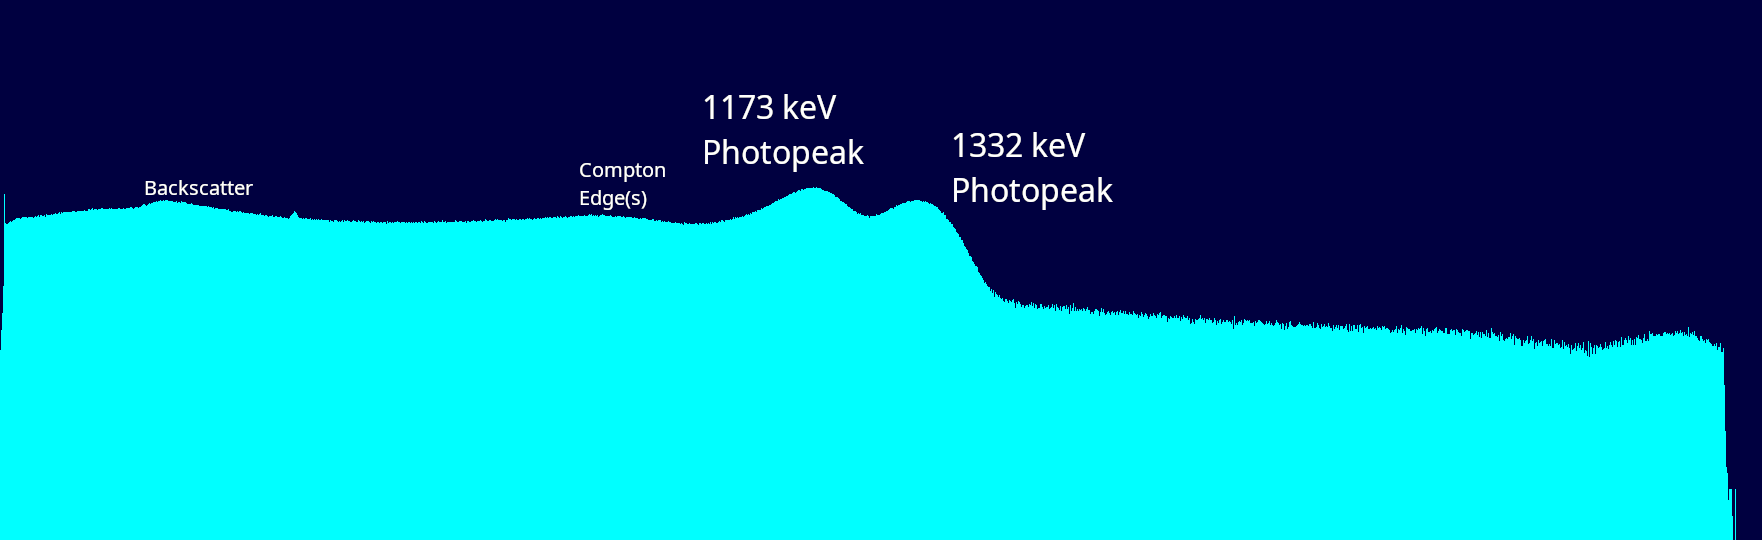
\includegraphics[scale=0.3]{assets/co60_log_annotated.png}
		\caption{Spectrum of Cobalt 60 - Log scale counts by energy}
	\end{figure}
	\begin{figure}[H] \centering
		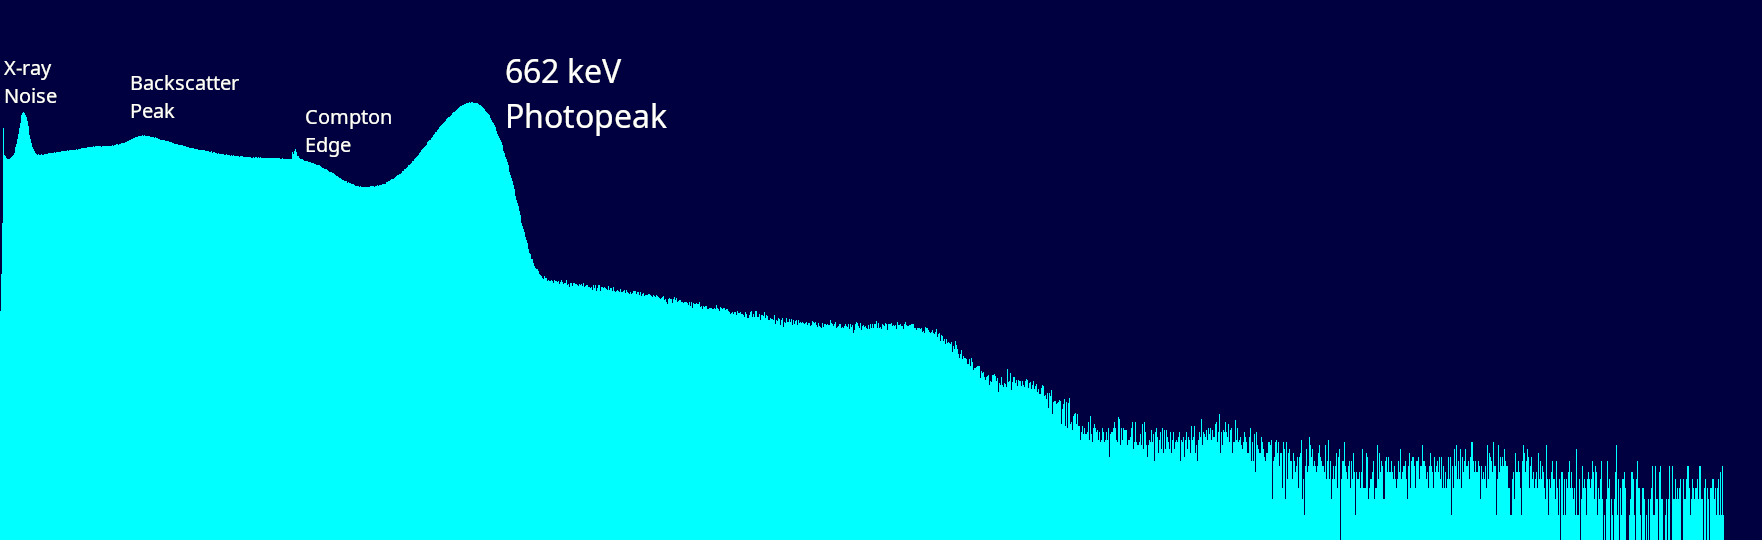
\includegraphics[scale=0.3]{assets/cs137_log_annotated.png}
		\caption{Spectrum of Cesium 137 - Log scale counts by energy}
	\end{figure}

\section{Source Strength Measurements}
	\dots

\section{Gamma Ray Absorption}
	It can be shown through a simple differential calculation that
	\begin{equation}
		I = I_0 e^{\frac{x}{\tau}}
	\end{equation}
	where $\tau$ is a function of the energy/wavelength of the photon. Therefore, by categorizing the data by photopeak energy and plotting the rate of detection by the thickness of the material for each separate material, we can calculate different values of $\tau$ and relate the absorption of the materials to each other.
	\begin{figure}[H] \centering
		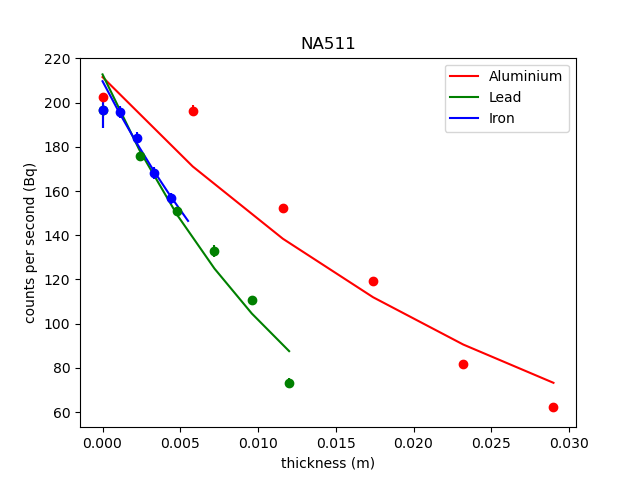
\includegraphics[scale=0.4]{assets/NA511.png}
		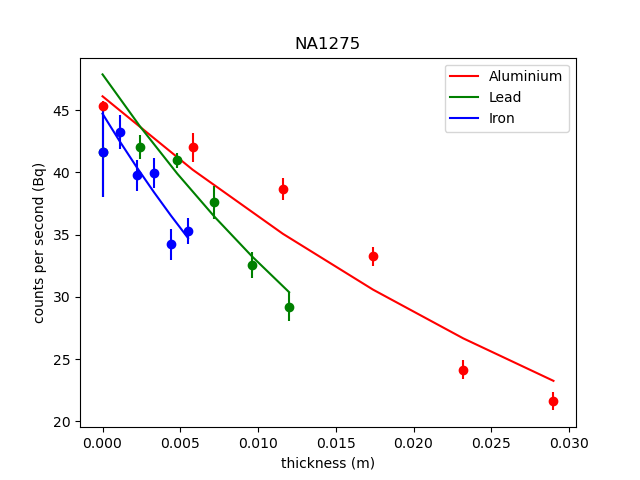
\includegraphics[scale=0.4]{assets/NA1275.png}
		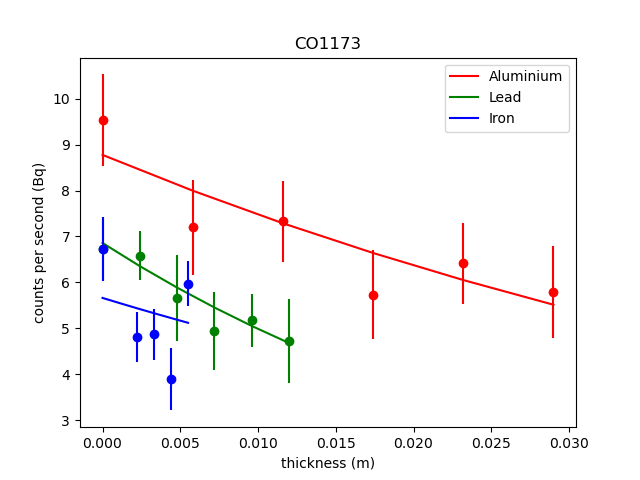
\includegraphics[scale=0.4]{assets/CO1173.png}
		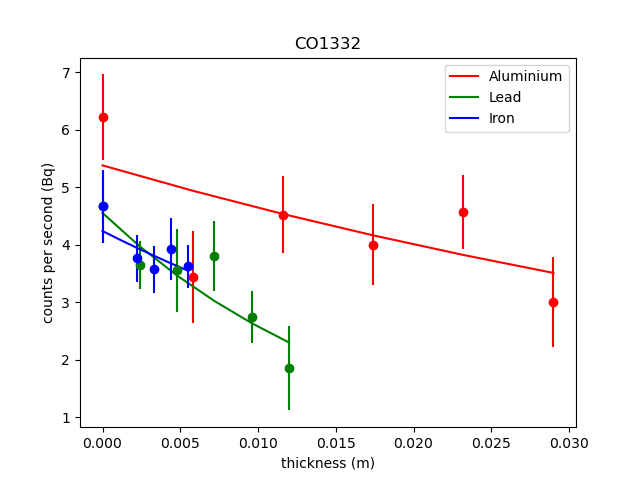
\includegraphics[scale=0.4]{assets/CO1332.png}
		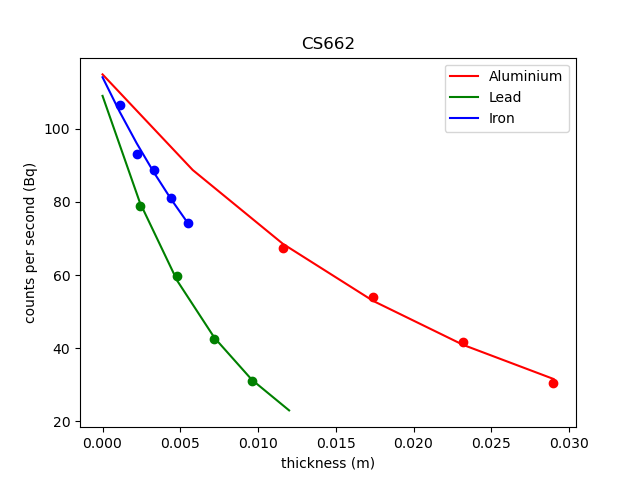
\includegraphics[scale=0.4]{assets/CS662.png}
		\caption{Counts per second measured for different thicknesses of different materials - each graph is of a different photopeak. Fit data shown below}
	\end{figure}

	\begin{center}
		\begin{tabular}{ ||c|c|c|c|c|c|| }
			$\tau$ & NA511 & NA1275 & CS662 & CO1173 & CO1332\\ 
			Aluminium & $0.027\pm0.002$ & $0.042\pm0.005$ & $0.022\pm0.003$ & $0.062\pm0.043$ & $0.068\pm0.047$\\
			Iron & $0.015\pm0.007$ & $0.022\pm0.015$ & $0.013\pm0.002$ & $0.055\pm0.125$ & $0.031\pm0.039$\\
			Lead & $0.014\pm0.002$ & $0.026\pm0.009$ & $0.008\pm0.001$ & $0.031\pm0.021$ & $0.018\pm0.006$\\
		\end{tabular}
		\begin{tabular}{ ||c|c|c|c|| }
			$\chi^2$ & Aluminium & Iron & Lead\\ 
			NA511 & $13.66$ & $0.14$ & $3.24$\\  
			NA1275 & $4.47$ & $0.49$ & $0.80$\\    
			CS662 & $0.39$ & $0.50$ & $0.24$\\    
			CO1173 & $0.59$ & $4.14$ & $0.23$\\    
			CO1332 & $3.03$ & $0.65$ & $2.34$\\    
		\end{tabular}
	\end{center}

\section{Data}
	Raw data is availible electronically[2].

\section{Analysis}
	analysis

\section{Conclusion}
	conclusion

\section*{References}

	\begin{hangparas}{.25in}{1}
		[1] Ocaya, Richard. (2006). An experiment to profile the voltage, current and temperature behaviour of a P-N diode. European Journal of Physics. 27. 625. 10.1088/0143-0807/27/3/015.
		
		[2] Daussy, C. et al. "Direct Determination of the Boltzmann Constant by an Optical Method". Phys. Rev. Lett. 98. (2007): 250801.
	\end{hangparas}

\end{document}
